\documentclass{standalone}
\usepackage{amssymb,amsmath}
\usepackage{tikz}
\usetikzlibrary{automata,positioning}
\begin{document}
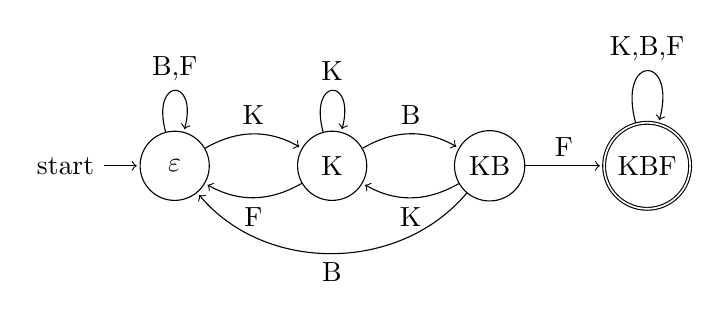
\begin{tikzpicture}[shorten >=1pt,node distance=2cm,on grid,auto] 
 \node[state,initial] (s_0) {$\varepsilon$};
 \node[state] (s_K)[right=of s_0] {K};
 \node[state] (s_KB)[right=of s_K] {KB};
 \node[state,accepting] (s_KBF)[right=of s_KB] {KBF};
 \path[->] 
 (s_0) edge [loop above] node {B,F} (s_0)
 (s_0) edge [bend left,above] node {K} (s_K)
 (s_K) edge [loop above] node {K} (K)
 (s_K) edge [bend left,above] node {B} (s_KB)
 (s_K) edge [bend left, below] node {F} (s_0)
 (s_KB) edge [bend left,below] node {K} (s_K)
 (s_KB) edge [bend left=50,below] node {B} (s_0)
 (s_KB) edge [above] node {F} (s_KBF)
 (s_KBF) edge [loop above] node {K,B,F} (s_KBF);
\end{tikzpicture} 
 \end{document}